\apendice{Especificación de diseño}

\section{Introducción}
En esta sección se mostrara el conjunto de diseños realizados para la correcta implementación del código. Para ello se distinguen de tres diseños:
\begin{itemize}
	\item \textbf{Diseño de datos}: En esta parte del diseño se mostrarán las estructuras de datos utilizadas.
	\item \textbf{Diseño procedimental}: En esta sección se mostraran diagramas relacionados con el flujo del programa.
	\item \textbf{Diseño arquitectonico}: En esta parte del diseño se especificará la arquitectura del proyecto.
\end{itemize}
\section{Diseño de datos}
Durante el desarrollo de la aplicación se trabajó con ficheros de datos que contenían una fila por cada fotograma del vídeo el cual a su vez contenía el número de fotograma los datos de las partes del cuerpo y los ángulos.

Para guardar los datos se ha implementado la persistencia utilizando dos bases de datos, dependiendo del entorno en el que se ejecute se utilizara una u otra. Si se ejecuta en el entorno de desarrollo se utiliza SQLite, si se ejecuta en el entorno de producción se utiliza PostgreSQL.

Para poder cumplir los requisitos de usuarios relacionados con la autenticación era necesario  almacenar los datos de los usuarios y sus credenciales encriptadas, para ello se creo dos tablas con una relación uno a uno, la tabla \textit{USER} y la tabla \textit{CREDENTIALS} estas se pueden ver en la figura \ref{fig:tablas-usuariocred}.

\begin{figure}
	\centering
	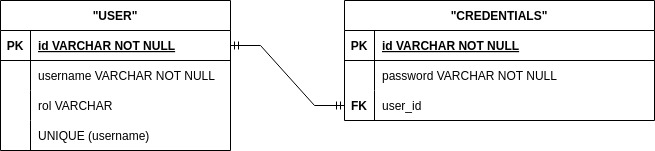
\includegraphics[width=0.7\linewidth]{img/tablas-UsuarioCred}
	\caption{Relación entre la tabla \textit{USER} y la tabla \textit{CREDENTIALS}.}
	\label{fig:tablas-usuariocred}
\end{figure}

Por otro lado, era necesario guardar los ejercicios con los que el usuario podrá comparar sus datos. Para ello se creó la tabla \textit{EXERCISE} que guardaba tanto el nombre del ejercicio como las rutas relativas de los ficheros de datos y de los vídeos. Como en la comparación de un ejercicio se pueden usar tanto las coordenadas de las posiciones del cuerpo como los ángulos, por ello se crearon dos tablas para guardar los nombres de las posiciones y de los ángulos, que fueron las tablas \textit{COORD} y \textit{ANGLE} respectivamente. Estas tablas tenían una relación muchos a muchos con la tabla \textit{EXERCISE}, por lo que se crearon dos tablas intermedias, como se puede observar en la figura \ref{fig:tablas-exercises}.

\begin{figure}
	\centering
	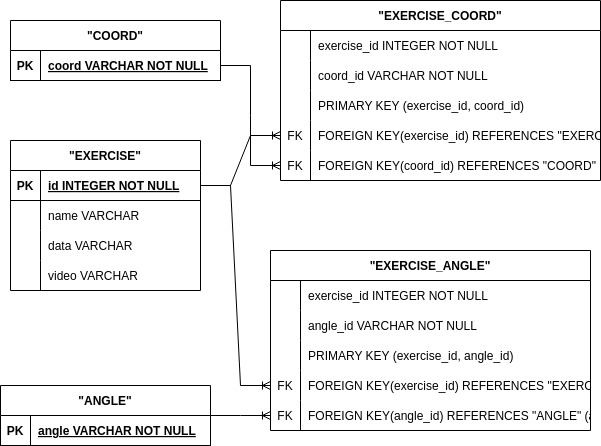
\includegraphics[width=0.7\linewidth]{img/tablas-Exercises}
	\caption{Diagrama relacional de las tablas referentes a los ejercicios.}
	\label{fig:tablas-exercises}
\end{figure}

\section{Diseño procedimental}
En este apartado se encuentra la explicación del flujo del programa durante su ejecución. En la figura \ref{fig:diagramasec} se mostrará el diagrama de secuencias de un usuario que va a usar la aplicación para obtener un puntuación de su vídeo. 
Como se puede observar, el usuario (habiendo iniciado sesión previamente) selecciona un ejercicio, lo que hace que se cargue la pagina con el vídeo del ejercicio, sube el fichero de datos de ese ejercicio y se compara con el fichero de datos 
\begin{figure}
	\centering
	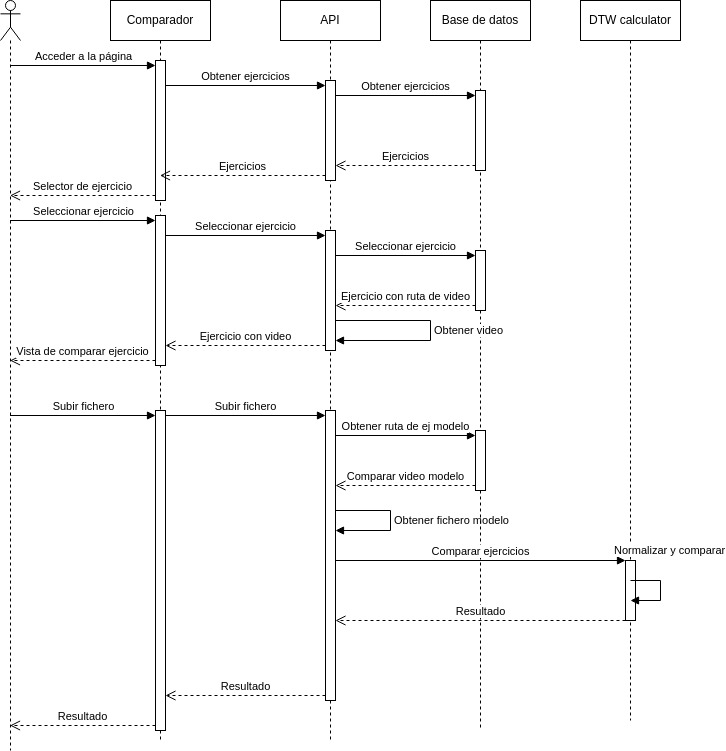
\includegraphics[width=0.7\linewidth]{img/diagramaSec}
	\caption{Diagrama de secuencia del flujo del paciente.}
	\label{fig:diagramasec}
\end{figure}

 
\section{Diseño arquitectónico}
La arquitectura de la aplicación consiste en dos paquetes, el \textit{backend} y el \textit{frontend}, ademas de la base de datos. 

La arquitectura usada ha sido el modelo multicapa, dividido en 4 capas~\cite{capas}:
\begin{enumerate}
	\item \textbf{Capa de presentación}: Es la interfaz de la aplicación, en este caso el \textit{frontend}.
	\item \textbf{Capa de aplicación o capa de servicios}: Es la fachada entre la capa de presentación y la capa de lógica de negocios, en este caso seria la API.
	\item \textbf{Capa de logica de negocio}: Se encarga tanto de la lógica de la aplicación como de gestionar los modelos.
	\item \textbf{Capa de origen de datos}: Se encarga de la persistencia de la aplicación, es decir las bases de datos.
\end{enumerate}


\begin{figure}
	\centering
	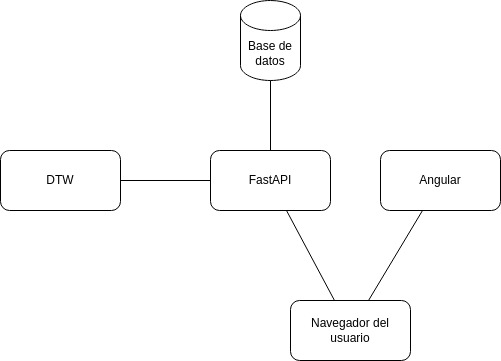
\includegraphics[width=0.7\linewidth]{img/DiagramaArq}
	\caption{Diagrama de la arquitectura.}
	\label{fig:diagramaarq}
\end{figure}

En el caso de que se despliegue la aplicación en mediante los contenedores de docker la aplicación constará de tres contenedores: el contenedor de la base de datos, el contenedor del \textit{backend}, que depende del de la base de datos, y el del \textit{frontend}.

